% -*- TeX -*-
%
% ----------------------------------------------------------------------
%
%                           Brad T. Aagaard
%                        U.S. Geological Survey
%
% {LicenseText}
%
% ----------------------------------------------------------------------
%
\documentclass[pdftex,cig,slideColor]{pp4slides}
\usepackage{amsmath}
\usepackage{array}
\usepackage{xspace}
\usepackage{multirow}
\usepackage{ulem}

\newcommand{\newfeature}[1]{{\color{blue}#1}}

\title{Finite-Element Modeling for Crustal Deformation}
\subtitle{}
\author{Brad Aagaard}
\institution{\includegraphics[height=2cm]{../../logos/cig}}
\date{June 14, 2010}

% --------------------------------------------------------- DOCUMENT
\begin{document}

% ------------------------------------------------------------ SLIDE
\maketitle
\vfill

% ------------------------------------------------------------ SLIDE
\foilhead{Crustal Deformation Modeling}
  \summary{Elasticity problems where geometry does not change significantly}

  \vfill
  Quasi-static modeling associated with earthquakes

  \begin{itemize}
  \item Strain accumulation associated with interseismic deformation
    \begin{itemize}
    \item What is the stressing rate on faults X, Y, and Z?
    \item Where is strain accumulating in the crust?
    \end{itemize}
  \item Coseismic stress changes and fault slip
    \begin{itemize}
    \item What was the slip distribution in earthquake A?
    \item How did earthquake A change the stresses on faults X, Y, and Z?
    \end{itemize}
  \item Post-seismic relaxation of the crust
    \begin{itemize}
    \item What rheology is consistent with observed post-seismic deformation?
    \item Can aseismic creep or afterslip explain the deformation?
    \end{itemize}
  \end{itemize}
  \vfill


\bgadd{\vspace*{7.9in}%
  \begin{center}%
    \includegraphics[height=14mm]{../../logos/cig}
  \end{center}}


% ------------------------------------------------------------ SLIDE
\foilhead{Crustal Deformation Modeling}
  \summary{Elasticity problems where geometry does not change significantly}

  \vfill
  Volcanic deformation associated with magma chambers and/or dikes
  \begin{itemize}
  \item Inflation
    \begin{itemize}
    \item What is the geometry of the magma chamber?
    \item What is the potential for an eruption?
    \end{itemize}
  \item Eruption
    \begin{itemize}
    \item Where is the deformation occurring?
    \item What is the ongoing potential for an eruption?
    \end{itemize}
  \item Dike intrusions
    \begin{itemize}
    \item What the geometry of the intrusion?
    \end{itemize}
  \end{itemize}
  \vfill


% ------------------------------------------------------------ SLIDE
\foilhead{Crustal Deformation Modeling}
  \summary{Overview of workflow for typical research problem}

  \vfill
  \begin{center}
    \includegraphics[scale=1.15]{figs/workflow}
  \end{center}
  \vfill

% ------------------------------------------------------------ SLIDE
\foilhead{Governing Equations}
  \summary{}

  \vfill
  Elasticity equation
  \begin{gather}
    \sigma_{ij,j} + f_i = \rho \ddot{u} \text{ in } V, \\
    \sigma_{ij} n_j = T_i \text{ on } S_T, \\
    u_i = u_i^0 \text{ on } S_u, \text{ and } \\
    R_{ki}(u^{+}_i - u^{-}_i) = d_k \text{ on } S_f.
  \end{gather}
  Multiply by weighting function and integrate over the volume,
  \begin{equation}
    -\int_V (\sigma_{ij,j} + f_i - \rho \ddot{u}_i) \phi_i \, dV = 0
  \end{equation}
  After some algebra,
  \begin{equation}
    -\int_V \sigma_{ij} \phi_{i,j} \, dV 
    + \int_{S_T} T_i \phi_i\, dS
    + \int_V f_i \phi_i \, dV 
    - \int_V \rho \ddot{u}_i \phi_i \, dV = 0
  \end{equation}
  \vfill
  
  
  
% ------------------------------------------------------------ SLIDE
\foilhead{Governing Equations}
  \summary{}

  \vfill
  Writing the trial and weighting functions in terms of basis (shape)
  functions,
  \begin{gather}
    u_i(x_i, t) = \sum_m a^m_i(t) N^m(x_i), \\
    \phi_i(x_i, t) = \sum_n c^n_i(t) N^n(x_i).
  \end{gather}
  After some algebra, the equation for vertex degree of freedom $i$ of
  vertex $n$ is
  \begin{multline}
    -\int_V \sigma_{ij} N^n_{,j} \, dV 
    + \int_{S_T} T_i N^n \, dS
    + \int_V f_i N^n \, dV 
    - \int_V \rho \sum_m \ddot{a}^m_i N^m N^n \, dV = 0
  \end{multline}
  \vfill

% ------------------------------------------------------------ SLIDE
\foilhead{Governing Equations}
  \summary{}

  Using numerical quadrature we convert the integrals to sums over the
  cells and quadrature points
  \begin{multline}
    -\sum_\text{vol cells} \sum_\text{quad pts} \sigma_{ij} N^n_{,j} w_q |J_\text{cell}|
    + \sum_\text{surf cells} \sum_\text{quad pts} T_i N^n w_q |J_\text{cell}|\\
    + \sum_\text{vol cells} \sum_\text{quad pts}  f_i N^n w_q |J_\text{cell}|\\
    - \sum_\text{vol cells} \sum_\text{quad pts} \rho \sum_m \ddot{a}^m_i N^m N^n w_q |J_\text{cell}| = \vec{0}    
  \end{multline}

% ------------------------------------------------------------ SLIDE
\foilhead{Quasi-static Solution}
  \summary{Neglect inertial terms}

  \vfill
  Form system of algebric equations
  \begin{equation}
    \underline{A} (t) \vec{u}(t) = \vec{b}(t)
  \end{equation}
  where
  \begin{gather}
    A^{nm}_{ij}(t) = \sum_\text{vol cells} \sum_\text{quad pts} 
      \frac{1}{4} C_{ijkl}(t) (N^m_{,l} + N^m_{,k})(N^n_{,j} + N^n_{,i}) w_q |J_\text{cell}| \\
    b_i(t) =    
     \sum_\text{surf cells} \sum_\text{quad pts} T_i(t) N^n w_q |J_\text{cell}| 
    + \sum_\text{vol cells} \sum_\text{quad pts}  f_i(t) N^n w_q |J_\text{cell}|
\end{gather}
  and solve for $\vec{u}(t)$.
  \vfill


% ------------------------------------------------------------ SLIDE
\foilhead{Problem Setup}
  \summary{}

  \begin{itemize}
  \item Which suite of tools should I use?
    \begin{itemize}
    \item Is there an analytic or semi-analytic solution?
    \item Can I solve a 2-D problem or do I need to solve a 3-D problem?
    \end{itemize}
  \item Which cell type is appropriate?
    \begin{itemize}
    \item Can I mesh the geometry of the domain with hexahedral cells?
    \item How will the discretization size vary in space?
    \end{itemize}
  \item What factors will control the resolution that I need?
    \begin{itemize}
    \item What length scales are important in my problem?
    \item What time scales are important?
    \end{itemize}
  \end{itemize}


% ------------------------------------------------------------ SLIDE
\foilhead{Basis Functions}
  \summary{$\vec{u}(\vec{x}, t) = \sum_n N^n(\vec{x}) \vec{u}^n(t)$}

  \vfill
 \begin{minipage}{3.0in}
    \begin{center}
      Triangle (3 basis fns)\\
      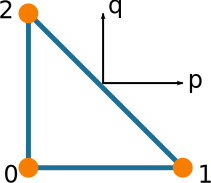
\includegraphics{figs/cell_tri3}
    \end{center}
    \begin{align*}
      N_0 &= \frac{1}{2}(-p-q) \\
      N_1 &= \frac{1}{2}(1+p) \\
      N_2 &= \frac{1}{2}(1+q)
    \end{align*}
  \end{minipage}
  \hfill
  \begin{minipage}{5.8in}
    \begin{center}
      Quadrilateral (4 basis fns)\\
      \includegraphics{figs/cell_quad4}
    \end{center}
    \begin{minipage}{2.7in}
      \begin{align*}
        N_3 &= \frac{1}{4}(1-p)(1+q) \\
        N_0 &= \frac{1}{4}(1-p)(1-q) 
      \end{align*}
    \end{minipage}
    \hfill
    \begin{minipage}{2.7in}
      \begin{align*}
        N_2 &= \frac{1}{4}(1+p)(1+q) \\
        N_1 &= \frac{1}{4}(1+p)(1-q)
     \end{align*}
    \end{minipage}
  \end{minipage}

  
% ------------------------------------------------------------ SLIDE
\foilhead{Varying Cell Size}
  \summary{}

  \begin{minipage}{4in}
    \begin{center}
      Stair-step\\
      \includegraphics[scale=0.4]{figs/tri3_step}\\
      \includegraphics[scale=0.4]{figs/quad4_step}
    \end{center}
  \end{minipage}
  \hfill
  \begin{minipage}{4in}
    \begin{center}
      Smooth\\
      \includegraphics[scale=0.4]{figs/tri3_smooth}\\
      \includegraphics[scale=0.4]{figs/quad4_smooth}
    \end{center}  
  \end{minipage}

  
% ------------------------------------------------------------ SLIDE
\foilhead{Potential Pitfalls}
  \summary{}

  \begin{itemize}
  \item Over/under resolving the deformation
    \begin{itemize}
    \item Poor mesh quality
    \item Using resolution much finer than constraints
    \item Failing to resolve stress concentrations
    \end{itemize}
  \item Failing to check the simulation results against intuition
    \begin{itemize}
    \item Do the results make sense?
    \item How close are the results to an anlytical solution?
    \end{itemize}
  \item Choosing the wrong suite of tools or parameters
    \begin{itemize}
    \item Nonlinear problems require nonlinear solvers
    \item Propagating seismic waves require inertial terms
    \end{itemize}
  \end{itemize}

% ------------------------------------------------------------ SLIDE
\foilhead{Poor Mesh Quality}
  \summary{Distorted cells}

  \vfill 
  The most distorted cell controls the rate convergence
  (quasi-static problems) and the time step (dynamic problems).
  \vfill

  \begin{center}
    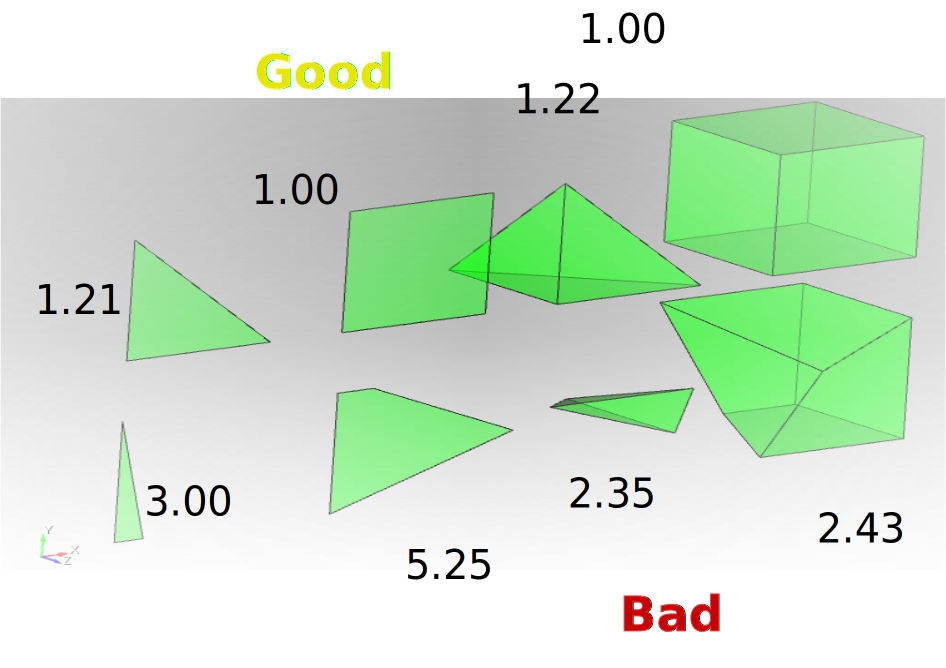
\includegraphics[scale=0.5]{figs/cells_distorted}
 \end{center}
  \vfill


% ------------------------------------------------------------ SLIDE
\foilhead{Hints, Tips, and Tricks}
  \summary{}

  \begin{itemize}
  \item Start at the coarsest resolution possible
  \item Work through the entire problem at a coarse resolution
    \begin{itemize}
    \item Eliminate obstacles using simple test problems that
      run quickly
    \item Verify workflow is feasible and meets desired objective
    \end{itemize}
  \item Increase resolution as needed
    \begin{itemize}
    \item Only run large problems when the kinks are worked out
    \item Verify solution is converging
    \end{itemize}
  \item Double-check inputs and outputs at every stage
    \begin{itemize}
    \item Did the software do what I think I told it to do?
    \end{itemize}  
  \end{itemize}

  
% ======================================================================
\end{document}


% End of file
